\section{Прямоугольная диаграмма}
Прямоугольная диаграмма - это плоская диаграмма, преобразованная простыми деформациями к такому виду, что все линии диаграммы идут по вертикали или по горизонтали, причём вертикальные линии проходят над горизонтальными.
Кроме того, есть соглашение, что линии диаграммы не должны принадлежать одной прямой.

\begin{tabular}{
>{\centering\arraybackslash}m{3cm}
>{\centering\arraybackslash}m{3cm}
>{\centering\arraybackslash}m{3cm}
>{\centering\arraybackslash}m{3cm}
}
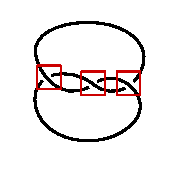
\includegraphics{images/sample-simple-knot-to-rect-0.pdf}
&
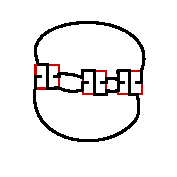
\includegraphics{images/sample-simple-knot-to-rect-1.pdf}
&
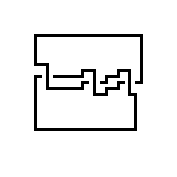
\includegraphics{images/sample-simple-knot-to-rect-2.pdf}
&
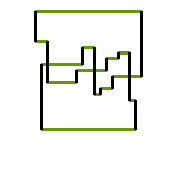
\includegraphics{images/sample-simple-knot-to-rect-4.pdf}
\\
Вокруг каждого пересечения выбрать прямоугольную окрестность, внутри которой нет никаких других линий.
&
Повернуть линии, проходящие внутри окрестности, а соединение их с внешними линиями линий провести по её границе.
&
Заменить плавные линии ступенчатыми ломаными
&
Передвинуть каждую линию на свою прямую.
Целесообразно вместо обозначений проход-переход обозначать верхние и нижние линии разным цветом.
\end{tabular}


Над прямоугольной диаграммой можно совершить следующие преобразования:
\begin{itemize}
\item Рокировка - перемена мест линий, если они при движении не зацепляются. Под зацеплением понимается заметание одного конца линии площадью, описываемой движением другой.

\begin{tabular}{
>{\centering\arraybackslash}m{3cm}
c
>{\centering\arraybackslash}m{3cm}
l
}
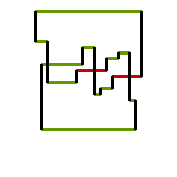
\includegraphics{images/rect-move-0.pdf}
&
$\rightarrow$
&
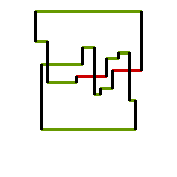
\includegraphics{images/rect-move-1.pdf}
&
Звенья совсем не касаются друг друга
\\
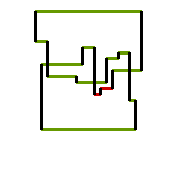
\includegraphics{images/rect-move-2.pdf}
&
$\rightarrow$
&
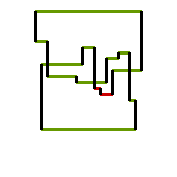
\includegraphics{images/rect-move-3.pdf}
&
Звенья касаются вершинами
\\
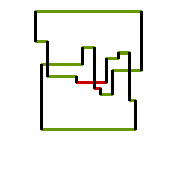
\includegraphics{images/rect-move-4.pdf}
&
$\rightarrow$
&
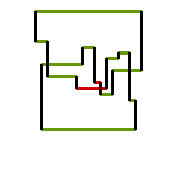
\includegraphics{images/rect-move-5.pdf}
&
Одно звено заметает обе вершины другого
\end{tabular}

\item Циклический перенос - перенос крайней линии через всю диаграмму на противоположный край.

\begin{tabular}{
>{\centering\arraybackslash}m{3cm}
c
>{\centering\arraybackslash}m{3cm}
}
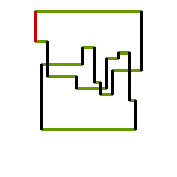
\includegraphics{images/rect-move-6.pdf}
&
$\rightarrow$
&
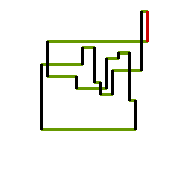
\includegraphics{images/rect-move-7.pdf}
\end{tabular}

Анвлогично можно переносить крайнюю линию сверху вниз, снизу вверх и справа налево.

\item Объединение линии - уничтожение минимальной ступеньки.
Если между соседними линиями есть ступенька, то её можно уничтожить, и две линии станут одной.

\begin{tabular}{
>{\centering\arraybackslash}m{3cm}
c
>{\centering\arraybackslash}m{3cm}
}
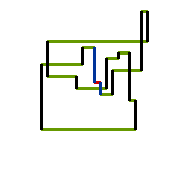
\includegraphics{images/rect-move-8.pdf}
&
$\rightarrow$
&
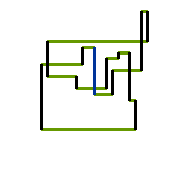
\includegraphics{images/rect-move-9.pdf}
\end{tabular}



\end{itemize}

По теореме, доказанной Дынниковым, любой тривиальный узел полумонотонно упрощается при помощи перечисленных преобразований.

Чтобы преобразовать плоскую диаграмму в вертикальную, нужно 1) каждое пересечение повернуть так, чтобы проходящая линия была расположена горизонтально, а переходящая - вертикально; 2) плавные и наклонные линии аппроксимировать ступенчатыми ломаными; 3) передвинуть каждое звено на свою прямую. Все эти операции должны делаться таким образом, чтобы не создавать новых пересечений.